\documentclass[11pt,a4paper]{article}

% Packages
\usepackage[utf8]{inputenc}
\usepackage[T1]{fontenc}
\usepackage{lmodern}
\usepackage[margin=1in]{geometry}
\usepackage{graphicx}
\usepackage{amsmath,amssymb}
\usepackage{booktabs}
\usepackage{hyperref}
\usepackage{xcolor}
\usepackage{listings}
\usepackage{algorithm}
\usepackage{algpseudocode}
\usepackage{tikz}
\usepackage{float}
\usetikzlibrary{shapes,arrows,positioning,fit,backgrounds}

% Colors
\definecolor{accent}{RGB}{59,130,246}
\definecolor{supports}{RGB}{34,197,94}
\definecolor{contradicts}{RGB}{239,68,68}
\definecolor{codebg}{RGB}{30,41,59}

% Hyperref setup
\hypersetup{
    colorlinks=true,
    linkcolor=accent,
    urlcolor=accent,
    citecolor=accent
}

% Code listing style
\lstset{
    backgroundcolor=\color{codebg},
    basicstyle=\ttfamily\small\color{white},
    breaklines=true,
    frame=single,
    rulecolor=\color{gray},
}

% Title
\title{
    \vspace{-1cm}
    \textbf{MedTrust AI: An Epistemology Layer for \\Medical Question Answering Systems}\\[0.5em]
    \large Transparent Evidence Attribution, Confidence Estimation, and Knowledge Gap Detection
}

\author{
    Rahul Kumar\\
    \texttt{github.com/rahul7932/healthtech-1}
}

\date{\today}

\begin{document}

\maketitle

\begin{abstract}
Large Language Models (LLMs) augmented with Retrieval-Augmented Generation (RAG) have shown promise in medical question answering. However, these systems typically produce opaque answers without transparent evidence attribution, confidence quantification, or acknowledgment of knowledge limitations. We present \textbf{MedTrust AI}, a post-hoc verification framework that adds an ``epistemology layer'' to medical RAG systems. Our approach decomposes generated answers into atomic claims, scores each claim against retrieved evidence, computes evidence-based confidence metrics, and systematically identifies knowledge gaps. The system produces a structured \textit{Trust Report} that enables clinicians and researchers to evaluate answer reliability at a granular level. We describe the architecture, methodology, and implementation of this system, demonstrating how transparent AI reasoning can bridge the gap between LLM capabilities and the rigorous evidentiary standards required in medical practice.
\end{abstract}

\section{Introduction}

\subsection{The Problem with Medical AI}

The integration of artificial intelligence into clinical decision support represents one of healthcare's most promising frontiers. Large Language Models, particularly when combined with Retrieval-Augmented Generation (RAG), can synthesize vast amounts of medical literature to answer complex clinical questions. However, a fundamental problem persists: \textbf{these systems provide answers without explaining their epistemic basis}.

Consider a typical RAG system responding to the question: ``Do ACE inhibitors reduce mortality in heart failure patients?'' The system retrieves relevant PubMed abstracts, feeds them to an LLM, and produces a fluent, authoritative-sounding answer. But critical questions remain unanswered:

\begin{itemize}
    \item Which specific passages support which specific claims?
    \item How strongly does the evidence support the conclusions?
    \item Are there contradicting studies the system considered?
    \item What clinically relevant factors are \textit{not} addressed by the evidence?
\end{itemize}

This opacity is particularly problematic in medicine, where practitioners are trained to evaluate evidence quality, consider alternative hypotheses, and acknowledge uncertainty. A system that cannot articulate \textit{why} it believes something is fundamentally incompatible with evidence-based medical practice.

\subsection{Our Contribution}

We introduce \textbf{MedTrust AI}, a verification framework that transforms opaque RAG outputs into transparent, auditable trust reports. Rather than replacing the RAG pipeline, our system operates as a \textit{post-hoc verification layer} that:

\begin{enumerate}
    \item \textbf{Extracts atomic claims} from generated answers
    \item \textbf{Attributes each claim} to supporting, contradicting, or neutral evidence
    \item \textbf{Computes confidence scores} based on evidence agreement and source diversity
    \item \textbf{Detects knowledge gaps} by identifying clinically relevant uncertainties
\end{enumerate}

The output is a structured \textit{Trust Report} that provides granular insight into the evidentiary basis of every claim—enabling users to make informed decisions about answer reliability.

\section{Background and Related Work}

\subsection{Retrieval-Augmented Generation}

RAG systems \cite{lewis2020retrieval} address LLM hallucination by grounding generation in retrieved documents. The standard pipeline consists of:

\begin{enumerate}
    \item \textbf{Query embedding}: Convert the user question to a vector representation
    \item \textbf{Retrieval}: Find semantically similar documents using vector similarity search
    \item \textbf{Generation}: Condition the LLM on retrieved passages to produce an answer
\end{enumerate}

While effective at reducing factual errors, standard RAG provides no mechanism for \textit{explaining} how retrieved evidence relates to generated claims.

\subsection{Citation and Attribution}

Recent work has explored inline citation generation, where models are prompted to cite sources within their responses. Systems like Bing Chat and Perplexity AI demonstrate this approach. However, these citations typically indicate which documents were \textit{consulted}, not whether they \textit{support} the specific claim being made—a crucial distinction in medical contexts.

\subsection{Confidence Estimation}

Traditional approaches to LLM confidence rely on token-level probabilities (logprobs). However, these reflect \textit{model certainty about word choice}, not \textit{epistemic confidence in factual claims}. A model may be highly confident in generating a grammatically correct but factually unsupported statement.

\subsection{The Gap: Epistemic Transparency}

Existing systems lack what we term \textbf{epistemic transparency}—the ability to articulate:
\begin{itemize}
    \item The relationship between evidence and conclusions
    \item The strength and limitations of that evidence
    \item What the system \textit{doesn't know}
\end{itemize}

MedTrust AI addresses this gap directly.

\section{System Architecture}

\subsection{Overview}

MedTrust AI operates as a verification layer atop a standard RAG pipeline. The complete system consists of six components executed sequentially:

\begin{figure}[H]
\centering
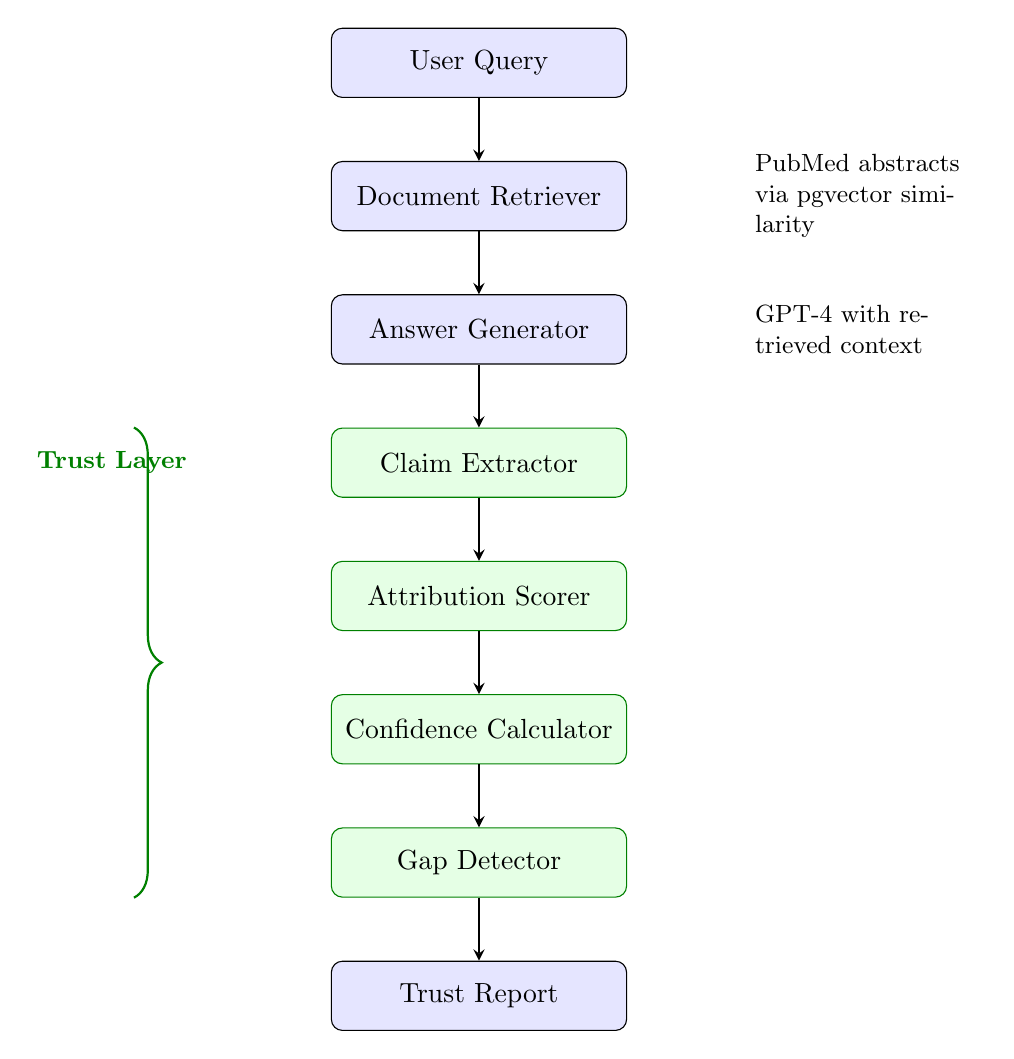
\begin{tikzpicture}[
    node distance=0.8cm,
    block/.style={rectangle, draw, fill=blue!10, text width=10em, text centered, rounded corners, minimum height=2.5em},
    trust/.style={rectangle, draw, fill=green!10, text width=10em, text centered, rounded corners, minimum height=2.5em, draw=green!50!black},
    arrow/.style={->, >=stealth, thick}
]

% Nodes
\node[block] (query) {User Query};
\node[block, below=of query] (retriever) {Document Retriever};
\node[block, below=of retriever] (generator) {Answer Generator};
\node[trust, below=of generator] (extractor) {Claim Extractor};
\node[trust, below=of extractor] (scorer) {Attribution Scorer};
\node[trust, below=of scorer] (confidence) {Confidence Calculator};
\node[trust, below=of confidence] (gaps) {Gap Detector};
\node[block, below=of gaps] (report) {Trust Report};

% Labels
\node[right=1.5cm of retriever, text width=8em, font=\small] {PubMed abstracts via pgvector similarity};
\node[right=1.5cm of generator, text width=8em, font=\small] {GPT-4 with retrieved context};
\node[left=1.5cm of extractor, text width=6em, font=\small, color=green!50!black] {\textbf{Trust Layer}};

% Arrows
\draw[arrow] (query) -- (retriever);
\draw[arrow] (retriever) -- (generator);
\draw[arrow] (generator) -- (extractor);
\draw[arrow] (extractor) -- (scorer);
\draw[arrow] (scorer) -- (confidence);
\draw[arrow] (confidence) -- (gaps);
\draw[arrow] (gaps) -- (report);

% Bracket for trust layer
\draw[decorate, decoration={brace, amplitude=10pt}, green!50!black, thick] 
    ([xshift=-2.5cm]extractor.north west) -- ([xshift=-2.5cm]gaps.south west);

\end{tikzpicture}
\caption{MedTrust AI system architecture. The Trust Layer (green) operates post-hoc on the RAG output.}
\label{fig:architecture}
\end{figure}

\subsection{Component 1: Document Retriever}

The retriever fetches relevant medical literature from a PostgreSQL database with pgvector extension. Documents are sourced from PubMed via the E-utilities API and embedded using OpenAI's \texttt{text-embedding-3-small} model (1536 dimensions).

Given a query $q$, retrieval proceeds as:
\begin{align}
    \mathbf{e}_q &= \text{embed}(q) \\
    D_k &= \underset{d \in \mathcal{D}}{\text{top-}k} \left( \text{cosine\_sim}(\mathbf{e}_q, \mathbf{e}_d) \right)
\end{align}

where $\mathcal{D}$ is the document corpus and $D_k$ is the set of $k$ most similar documents.

\subsection{Component 2: Answer Generator}

The generator produces a synthesized answer conditioned on retrieved documents. We use GPT-4 with a system prompt requiring inline citations in the format \texttt{[PMID:xxxxx]}:

\begin{lstlisting}
You are a medical research assistant. Answer based 
ONLY on the provided evidence. Cite sources inline 
using [PMID:xxxxx] format. If evidence is insufficient, 
say so explicitly.
\end{lstlisting}

\subsection{Component 3: Claim Extractor}

The claim extractor decomposes the generated answer into atomic, verifiable claims. This is critical because:

\begin{itemize}
    \item Paragraphs contain multiple distinct assertions
    \item Evidence may support some claims but not others
    \item Confidence varies at the claim level, not the answer level
\end{itemize}

We use structured output via the Instructor library to ensure consistent JSON formatting:

\begin{lstlisting}
{
  "claims": [
    {
      "id": "claim_1",
      "text": "ACE inhibitors reduce mortality",
      "span_start": 0,
      "span_end": 31
    },
    ...
  ]
}
\end{lstlisting}

The \texttt{span\_start} and \texttt{span\_end} fields enable highlighting claims in the original answer.

\subsection{Component 4: Attribution Scorer}

For each claim-document pair $(c_i, d_j)$, the attribution scorer determines the evidential relationship:

\begin{equation}
    \text{attribution}(c_i, d_j) \in \{\textsc{supports}, \textsc{contradicts}, \textsc{neutral}\}
\end{equation}

This is implemented via LLM classification with the prompt:

\begin{lstlisting}
Given this claim and this passage, classify their 
relationship as:
- SUPPORTS: passage provides evidence for the claim
- CONTRADICTS: passage provides evidence against
- NEUTRAL: passage neither supports nor contradicts
\end{lstlisting}

The result is a complete evidence map: each claim is associated with lists of supporting, contradicting, and neutral documents.

\subsection{Component 5: Confidence Calculator}

Unlike logprob-based confidence, our approach computes \textbf{evidence-based confidence}:

\begin{equation}
    \text{confidence}(c_i) = \text{agreement}(c_i) \times \log(1 + |S_i|) \times w_{\text{quality}}
\end{equation}

where:
\begin{itemize}
    \item $\text{agreement}(c_i) = \frac{|S_i| - |C_i|}{|S_i| + |C_i| + \epsilon}$ measures evidence consensus
    \item $|S_i|$ and $|C_i|$ are counts of supporting and contradicting documents
    \item $w_{\text{quality}}$ is a weighting factor based on study type (RCT $>$ observational)
\end{itemize}

This formulation captures three intuitions:
\begin{enumerate}
    \item Claims with contradicting evidence should have lower confidence
    \item Claims supported by more independent sources are more reliable
    \item Evidence quality matters (though current implementation uses uniform weights)
\end{enumerate}

Overall confidence is the mean across all claims:
\begin{equation}
    \text{confidence}_{\text{overall}} = \frac{1}{n} \sum_{i=1}^{n} \text{confidence}(c_i)
\end{equation}

\subsection{Component 6: Gap Detector}

The gap detector identifies \textbf{what the evidence does not address}. For each claim, we prompt the LLM:

\begin{lstlisting}
Given this claim and its supporting evidence, identify 
clinically relevant factors that are NOT addressed:
- Patient populations not covered
- Dosing/duration uncertainties  
- Long-term outcomes not studied
- Relevant comorbidities not considered
\end{lstlisting}

This mimics the clinical reasoning process where practitioners identify limitations in the evidence base.

Global gaps are aggregated across all claims to identify systematic knowledge limitations.

\section{The Trust Report}

The output of MedTrust AI is a structured Trust Report containing:

\begin{lstlisting}
{
  "query": "...",
  "answer": "...",
  "claims": [
    {
      "id": "claim_1",
      "text": "...",
      "supporting_docs": [...],
      "contradicting_docs": [...],
      "neutral_docs": [...],
      "confidence": 0.72,
      "missing_evidence": [...]
    }
  ],
  "overall_confidence": 0.68,
  "evidence_summary": {
    "total_sources": 5,
    "supporting": 3,
    "contradicting": 1,
    "neutral": 1
  },
  "global_gaps": [...]
}
\end{lstlisting}

This structure enables:
\begin{itemize}
    \item \textbf{Claim-level inspection}: Users can examine evidence for specific assertions
    \item \textbf{Conflict identification}: Contradicting studies are explicitly surfaced
    \item \textbf{Confidence interpretation}: Scores reflect evidence strength, not model certainty
    \item \textbf{Limitation awareness}: Knowledge gaps are systematically documented
\end{itemize}

\section{Implementation}

\subsection{Technology Stack}

\begin{table}[H]
\centering
\begin{tabular}{ll}
\toprule
\textbf{Component} & \textbf{Technology} \\
\midrule
Backend Framework & FastAPI (Python) \\
Database & PostgreSQL + pgvector (Supabase) \\
Embeddings & OpenAI text-embedding-3-small \\
LLM & GPT-4o \\
Frontend & React + TypeScript + Tailwind CSS \\
Structured Output & Instructor library \\
\bottomrule
\end{tabular}
\caption{Technology stack}
\end{table}

\subsection{Data Pipeline}

\begin{enumerate}
    \item \textbf{Ingestion}: PubMed abstracts are fetched via E-utilities API
    \item \textbf{Embedding}: Title + abstract are embedded and stored in pgvector
    \item \textbf{Retrieval}: Cosine similarity search returns top-k documents
    \item \textbf{Processing}: Trust Layer components execute sequentially
    \item \textbf{Presentation}: React dashboard visualizes the Trust Report
\end{enumerate}

\subsection{Performance Considerations}

The Trust Layer introduces latency due to multiple LLM calls:
\begin{itemize}
    \item Claim extraction: 1 call
    \item Attribution scoring: $O(n \times k)$ calls (claims $\times$ documents)
    \item Gap detection: $O(n)$ calls
\end{itemize}

For a typical query with 10 claims and 5 documents, this results in approximately 60 LLM calls. We mitigate this through:
\begin{itemize}
    \item Parallel execution where dependencies allow
    \item Caching of document embeddings
    \item Batched attribution scoring (future work)
\end{itemize}

\section{Discussion}

\subsection{Why This Matters}

MedTrust AI addresses a fundamental tension in medical AI: the need for both \textbf{capability} (answering complex questions) and \textbf{accountability} (explaining reasoning). Our system demonstrates that these goals are not mutually exclusive.

Key implications:

\begin{enumerate}
    \item \textbf{Clinical Decision Support}: Practitioners can evaluate AI recommendations against the same evidentiary standards they apply to human colleagues.
    
    \item \textbf{Medical Education}: Students can see how conclusions are derived from literature, reinforcing evidence-based reasoning skills.
    
    \item \textbf{Research Synthesis}: Researchers can quickly identify gaps in the evidence base for specific clinical questions.
    
    \item \textbf{Regulatory Compliance}: Transparent reasoning supports audit requirements for AI-assisted clinical decisions.
\end{enumerate}

\subsection{Limitations}

\begin{itemize}
    \item \textbf{LLM Dependence}: Attribution scoring relies on LLM judgment, which may itself be imperfect.
    
    \item \textbf{Literature Coverage}: Quality depends on the underlying document corpus; rare conditions may have insufficient coverage.
    
    \item \textbf{Latency}: Multiple LLM calls introduce significant processing time.
    
    \item \textbf{Study Quality}: Current implementation does not weight RCTs over observational studies.
\end{itemize}

\subsection{Future Work}

\begin{itemize}
    \item \textbf{Evidence Quality Weighting}: Incorporate study design hierarchy (systematic reviews $>$ RCTs $>$ cohort studies)
    
    \item \textbf{Temporal Awareness}: Weight recent evidence more heavily; flag outdated guidelines
    
    \item \textbf{Contradiction Resolution}: When evidence conflicts, explain possible reasons (different populations, methodologies)
    
    \item \textbf{Fine-tuned Attribution}: Train specialized models for medical evidence classification
\end{itemize}

\section{Conclusion}

MedTrust AI demonstrates that medical AI systems can provide not just answers, but \textbf{epistemically transparent reasoning}. By decomposing answers into claims, attributing each to specific evidence, quantifying confidence based on evidence agreement, and systematically identifying knowledge gaps, our system bridges the gap between LLM capabilities and the rigorous standards of evidence-based medicine.

The Trust Report format provides a structured interface for human oversight—enabling practitioners to leverage AI capabilities while maintaining the critical evaluation skills that define good medical practice.

As AI systems become more prevalent in healthcare, the ability to ``show your work'' will transition from a nice-to-have to a fundamental requirement. MedTrust AI offers a practical framework for achieving this goal.

\section*{Acknowledgments}

This project was developed as a demonstration of transparent medical AI reasoning. The system is intended for research and educational purposes and should not be used for clinical decision-making without appropriate validation.

\begin{thebibliography}{9}

\bibitem{lewis2020retrieval}
Lewis, P., et al. (2020). Retrieval-Augmented Generation for Knowledge-Intensive NLP Tasks. \textit{NeurIPS 2020}.

\bibitem{openai2023gpt4}
OpenAI. (2023). GPT-4 Technical Report. \textit{arXiv preprint arXiv:2303.08774}.

\bibitem{sackett1996evidence}
Sackett, D. L., et al. (1996). Evidence based medicine: what it is and what it isn't. \textit{BMJ}, 312(7023), 71-72.

\bibitem{topol2019high}
Topol, E. J. (2019). High-performance medicine: the convergence of human and artificial intelligence. \textit{Nature Medicine}, 25(1), 44-56.

\bibitem{johnson2023assessing}
Johnson, D., et al. (2023). Assessing the Accuracy and Reliability of AI-Generated Medical Responses. \textit{JAMA Internal Medicine}.

\end{thebibliography}

\end{document}
